\chapter{Sistema de Reconhecimento Facial Visage} \label{chap:visage}

Neste capítulo é apresentado o sistema de reconhecimento facial automático em imagens Visage.  Em primeiro lugar é abordada a motivação do estudo da aplicação de filtros de abstração em sistemas de reconhecimento facial tendo em conta o estado da arte reportado nos Capítulos \ref{chap:reco} e \ref{chap:abstracao}. Posteriormente, é apresentada uma visão geral do sistema de reconhecimento facial criado e das tecnologias utilizadas para sua implementação. Em terceiro lugar, encontra-se descrita a biblioteca de imagens utilizada como base para o desenvolvimento e avaliação do sistema Visage. De seguida, é apresentada arquitetura adotada neste sistema. A quinta e sexta secções deste capítulo descrevem pormenorizadamente os dois principais módulos que o compõem. Finalmente, em sétimo lugar, são apresentadas as principais funcionalidades do sistema desenvolvido.


\section{Filtros de Abstração de Imagens no Reconhecimento Facial}
O reconhecimento facial em imagens sofreu uma evolução notável nos últimos 20 anos, tal como documentado no Capítulo \ref{chap:reco}. 

Em cenários cooperativos com condições de captura de imagens controladas, nomeadamente ao nível da pose, iluminação e expressões faciais, considera-se mesmo que o problema de verificação 1:1 se encontra praticamente resolvido, uma vez que as taxas de reconhecimento atingidas são satisfatórias para a grande maioria das aplicações \cite{Li2011}. Existem também várias aplicações em situações reais com um bom nível de satisfação por parte dos seus utilizadores, como é o caso do sistema de fronteira automático dos aeroportos portugueses (ver \ref{CartoesInteligentes}), ou o controlo de entradas nas cerimónias inaugurais dos jogos olímpicos de Pequim (ver \ref{sec:SegurancaAplicaçãoLei}). Em condições específicas e favoráveis, é então possível considerar que os sistemas de reconhecimento facial automático atuais conseguem mesmo ultrapassar a capacidade de reconhecimento humana, uma vez que conseguem identificar com precisão um maior número de faces do que aquelas que um humano consegue.

Contudo, o problema de reconhecimento facial automático ainda se encontra longe de ser um problema totalmente resolvido. Em cenários onde é registada uma grande variação ao nível da pose, iluminação ou outros fatores identificados na Secção \ref{desafios}, a identificação das entidades capturadas é ainda uma área de investigação em aberto \cite{Li2011}. Para além disso, o desempenho e satisfação obtida por parte dos utilizadores dos sistemas atuais demonstra uma grande variação tendo em conta as situações onde estes sistemas são utilizados. 

Por outro lado, a crescente ubiquidade tecnológica e poder computacional presente nos diversos dispositivos utilizados no nosso dia a dia aumenta o leque de aplicações possíveis do reconhecimento facial automático, apresentando novos desafios às soluções atualmente existentes (ver \ref{sec:areasAplicacao}).

Considerando todos os fatores mencionados anteriormente , o elevado custo soluções comerciais existentes e ainda a falta soluções abertas, torna-se pertinente a realização de investigação na área do reconhecimento facial em imagens. 

Ao nível da abstração de imagens, estudos efetuados demonstraram que aplicação de filtros de abstração de imagens na recuperação de informação multimédia, nomeadamente no âmbito da da ilustração automática de texto, tem a potencialidade de melhorar a informação retornada, assim como reduzir significativamente as necessidades de processamento e armazenamento das imagens \cite{Coelho:2012:IAC:2260641.2260676}. 

Tendo em conta a importância e a necessidade de investigação na área do reconhecimento facial automático, e uma vez que não existem estudos relativos à utilização de filtros de abstração no processo de reconhecimento facial, torna-se pertinente o estudo do seu impacto. A hipótese levantada no âmbito desta dissertação é então que o uso da abstração em imagens que vão ser ser alvo de reconhecimento facial pode melhorar o processo de reconhecimento facial automático em imagens.

\section{Visage - Visão geral} \label{sec:visage}
A criação do sistema Visage teve como principal objetivo o desenvolvimento de um sistema de reconhecimento facial automático que permita analisar qual o impacto da abstração de imagens e outras tarefas de pré-processamento no processo de reconhecimento facial automático. Com o sistema desenvolvido pretende-se ainda a criação de uma base sólida que permita o desenvolvimento de futuras aplicações que tirem partido do reconhecimento facial automático no seu funcionamento, como por exemplo, aplicações na área de \textit{image retrieval}.

O sistema de reconhecimento facial desenvolvido é composto por um conjunto de aplicações que seguem um paradigma de caixa preta, no qual para um conjunto de dados de entrada é produzido um resultado específico. Um exemplo de um componente do sistema Visage desenvolvido segundo o paradigma caixa preta é a aplicação \textit{FaceDetector.exe}. Nesta aplicação para uma biblioteca de imagens fornecida como entrada é devolvida uma nova biblioteca sobre a qual foram aplicadas um conjunto de tarefas de pré-processamento sobre as imagens da mesma. As restantes aplicações que compõem o sistema desenvolvido encontram-se descritas na Secção \ref{sec:funcionalidades}.

De uma forma genérica, o funcionamento do sistema Visage pode ser agrupado nas seguintes fases fundamentais:
\begin{description}
\item[Pré-processamento] Corresponde à primeira etapa executada, na qual é fornecida uma galeria de imagens a pré-processar, as quais irão ser posteriormente utilizadas na fases de treino e identificação. O pré-processamento engloba tarefas como deteção das faces na imagem, normalização do contraste e iluminação, aplicação de filtros de abstração ou alinhamento das imagens.
\item[Treino] Nesta fase são fornecidas um conjunto de imagens anotadas ao sistema e pretende-se que este crie uma base de conhecimento que permita de futuro proceder à identificação de novas imagens de acordo com a informação treinada.
\item[Identificação] Corresponde à utilização do sistema como o intuito de identificar novas imagens não anotadas. Para uma dada imagem fornecida ao sistema, este deve devolver no nome da pessoa que se encontra na imagem tendo em conta a informação obtida na fase de treino. Nesta fase é também possível obter uma lista de entidades, ordenada de forma crescente pela similaridade em relação à pessoa representada na imagem.
\end{description}

Uma vez que o foco desta dissertação não é o desenvolvimento de algoritmos de reconhecimento facial, mas sim a análise do impacto da manipulação efetuada sobre as imagens a reconhecer, foram utilizadas bibliotecas de código aberto que fornecem a implementação de algoritmos bem estabelecidos para o reconhecimento facial automático e facilitam a manipulação efetuada sobre as imagens. Por outro lado, a utilização destas bibliotecas permite também a contribuição para uma área onde as soluções abertas existentes são ainda poucas.

Para a manipulação das imagens e implementação do sistema de reconhecimento facial foi utilizada a biblioteca \textit{Open Source Computer Vision Library} (\textit{OpenCV}), uma biblioteca de código aberto nas áreas de visão por computador e \textit{machine learning}, onde se encontram implementados mais de 2500 algoritmos relacionados com as áreas de computação gráfica e visão por computador. Esta biblioteca possui uma comunidade de mais do que 47 mil utilizadores, já registou mais de 5 milhões de downloads e é utilizada globalmente por empresas como a Google, Yahoo, Microsoft, Intel, IBM, Sony, Honda, Toyota \cite{Team}. Ao nível do reconhecimento facial, esta biblioteca disponibiliza um módulo denominado \textit{Face Recognizer}, onde se encontram implementados os algoritmos \textit{Eigenfaces}, \textit{Fisherfaces} e \textit{Local Binary Patterns Histograms}. Tendo em conta a ampla utilização da biblioteca OpenCV e a sua constante atualização pela comunidade, assim como as facilidades providenciadas pelo módulo de reconhecimento facial, esta foi considerada a biblioteca a utilizar como base de implementação do sistema de reconhecimento facial a criar.

Ao nível dos filtros de abstração foram utilizados os filtros gaussiano e bilateral, implementados na biblioteca \textit{OpenCV}, e ainda o filtro anisotrópico kuwahara, recorrendo para a sua utilização à implementação efetuada por Kyprianidis \textit{et al.} \cite{Kyprianidis2009} do mesmo filtro.

Finalmente, ao nível das galerias de imagens, foi utilizada a coleção \textit{Labeled Faces in the Wild} descrita na secção seguinte.


\section{Biblioteca de Dados - \textit{Labeled Faces in the Wild}} \label{sec:lfw}

A evolução do reconhecimento facial automático em imagens tem beneficiado do aumento dos recursos disponíveis para o seu estudo, nomeadamente através da criação de novas e mais completas coleções de dados \cite{Huang2007}. A grande maioria destas coleções caracteriza-se por ter condições de captura controladas, com o intuito de efetuar o estudo de fatores específicos que afetam a qualidade do reconhecimento. A análise do problema de reconhecimento facial automático de um ponto de vista geral implica a escolha de uma biblioteca apropriada e que represente a grande variabilidade associada aos diferentes desafios que afetam o reconhecimento facial em imagens.

Para o desenvolvimento do sistema de reconhecimento facial Visage e posterior análise dos resultados foi escolhida a biblioteca de imagens \textit{Labeled Faces in the Wild}.

A biblioteca \textit{Labeled Faces in the Wild (LFW)} é uma base de dados fotográfica desenhada especificamente para o estudo do problema de reconhecimento facial, particularmente em situações onde as condições de captura das imagens não possuem restrições. Nesse sentido, as imagens que constituem a galeria caracterizam-se por possuir uma grande variabilidade, nomeadamente ao nível da pose, expressão, iluminação, etnia, idade, género, vestuário e qualidade da câmara com a qual foi efetuada a captura \cite{Huang2007}.
\begin{figure}[ht]
  \begin{center}
    \leavevmode
    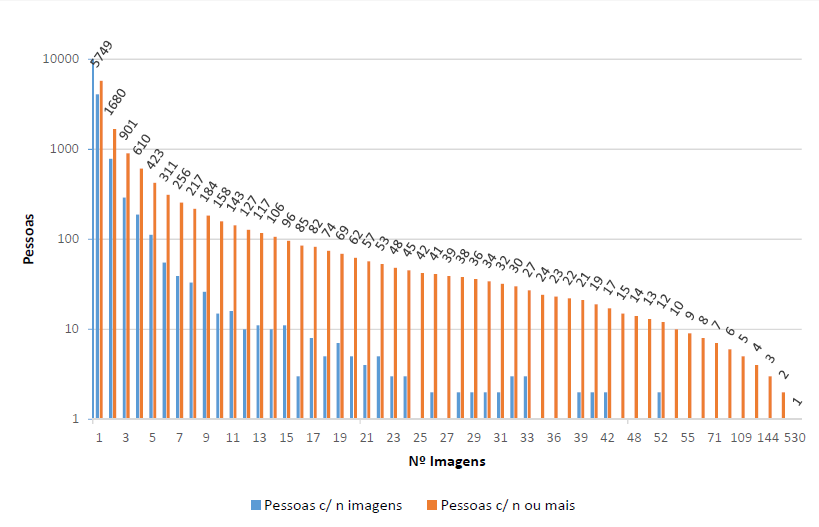
\includegraphics[width=1\textwidth]{Distribuicao}
    \caption{Distribuição do número de imagens por pessoa na biblioteca LFW.}
    \label{fig:distribuicaoLFW}
  \end{center}
\end{figure}
Nesta biblioteca encontram-se representados 5749 indivíduos, ilustrados por 13233 imagens. O número de imagens por pessoa apresenta no entanto uma grande variação, desde um mínimo de 1 imagem por pessoa para 4069 indivíduos, até um máximo de 530 imagens que representam o antigo presidente dos Estados Unidos da América George W. Bush. O gráfico na Figura \ref{fig:distribuicaoLFW} ilustra a grande variação da distribuição do número de imagens por pessoa. No eixo vertical encontram-se representadas o número de pessoas em escala logarítmica e no eixo horizontal o número de imagens correspondente.

Devido à inexistência de restrições na captura de imagens, cada fotografia pode possuir mais do que uma face representada, sendo que a face que contém o píxel central deve ser considerada como a entidade representada na imagem. As imagens desta biblioteca são maioritariamente a cores, com diferentes graus de saturação, existindo também um número reduzido de imagens a preto e branco. A cada imagem encontra-se também associada uma anotação textual, relativa ao nome da pessoa representada. A Tabela \ref{tab:lfw} sintetiza algumas das características mais significativas da biblioteca. Nesta tabela são reportadas as caraterísticas da biblioteca no formato de imagens PNG uma vez que este foi o formato utilizado para avaliação do impacto dos filtros de abstração no processo de reconhecimento.

\begin{center}
\begin{table}
	\caption{Caracterização da Biblioteca LFW}
	\begin{center}
    \begin{tabular}{ll}
    \hline
    Característica                            & Valor            \\ \hline
    Imagens                                   & 13233 imagens    \\
    Pessoas representadas                     & 5749 pessoas     \\
    Tamanho total                             & 1.18 GB          \\
    Formato                                   & PNG              \\
    Tamanho de cada imagem: min / médio / max & 46.49 KB/ 93.72 KB/ 147.89 KB\\
    Dimensões imagem                          & 250$\times$250 píxeis \\
    \hline
    \end{tabular}
	\label{tab:lfw}
	\end{center}
\end{table}
\end{center}

Para além da biblioteca LFW original, encontram-se também disponíveis para fins de investigação duas outras bibliotecas derivadas da biblioteca original, LFW funneled e LFW-a, onde as imagens originais foram sujeitas a um pré-processamento com vista a efetuar o alinhamento da posição da face na imagem, cada uma correspondendo a uma técnica diferente de alinhamento da imagem. Um exemplo de uma variante da mesma foto nas diferentes bibliotecas pode ser visto na Figura \ref{fig:lfwversoes}.

\begin{figure}[h]
        \centering
        \begin{subfigure}[b]{0.25\textwidth}
                \centering
                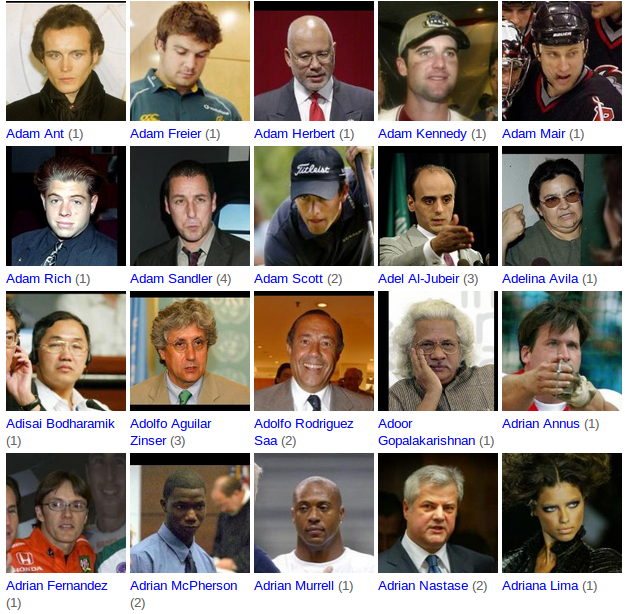
\includegraphics[width=\textwidth]{lfw_versoes/lfw}
                \caption{LFW}
                \label{fig:lfw_original}
        \end{subfigure}%
        ~ 
        \begin{subfigure}[b]{0.25\textwidth}
                \centering
                \includegraphics[width=\textwidth]{lfw_versoes/lfw-a}
                \caption{LFW-a}
                \label{fig:lfw_a}
        \end{subfigure}
        ~ 
        \begin{subfigure}[b]{0.25\textwidth}
                \centering
                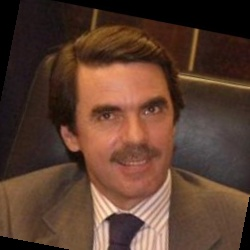
\includegraphics[width=\textwidth]{lfw_versoes/lfw-funneled}
                \caption{LFW funneled}
                \label{fig:lfw_funneled}
        \end{subfigure}
        \caption{Diferentes versões da biblioteca LFW}\label{fig:lfwversoes}
\end{figure}

A coleção LFW é particularmente interessante para o estudo do desempenho do sistema desenvolvido e consequentemente do impacto do uso da abstração de imagens no reconhecimento facial, uma vez que a variabilidade presente nas suas imagens, devido ao facto de estas não terem sido capturadas com o intuito específico da análise deste problema, representa uma amostra aproximada das variações encontradas no dia-a-dia de uma pessoa \cite{Huang2007}. Por outro lado, e uma vez que não pretendemos analisar a tarefa de alinhamento da face, a existência de versões já alinhadas da biblioteca permitiu retirar um fator importante de variação dos resultados obtidos. Assim sendo, optamos pela utilização da versão alinhada LFW-a para fins de avaliação do desempenho do sistema de reconhecimento facial criado e do impacto do uso de filtros de abstração no processo de reconhecimento.

\section{Arquitetura}
O sistema de reconhecimento facial criado é constituído pelos seguintes 6 módulos:

\begin{description}
\item[\textit{Person}] Módulo responsável por efetuar o encapsulamento da informação relativa a uma pessoa, nomeadamente o seu nome, código de identificação e imagens a esta associada. De modo a facilitar a avaliação do sistema criado é ainda possível armazenar de forma diferenciada imagens de treino e teste de cada pessoa.
\item[\textit{Library}]Módulo responsável por encapsular a informação de uma galeria de imagens utilizada para treinar o sistema, nomeadamente o seu diretório, as pessoas representadas nessa biblioteca (agrupadas num \textit{array} de objetos do tipo \textit{Person}) e alguns dados estatísticos como o número mínimo e máximo de imagens existentes por pessoa e o número total de imagens da galeria. Apesar de poder ser utilizado com diferentes funcionalidades este módulo foi desenvolvido com o intuito de facilitar a avaliação do sistema Visage com diferentes galerias de imagens, pelo que na criação de uma \textit{Library} é possível definir qual a percentagem das imagens, de cada pessoa, que devem ser utilizadas como conjunto de teste e conjunto de treino do sistema (Ver Capítulo \ref{chap:resultados} para mais detalhes).
\item[\textit{FaceDetector}] A par do módulo \textit{FaceModel} é um dos componentes principais do sistema, sendo responsável por efetuar um conjunto de tarefas de pré-processamento sobre as imagens utilizadas. Este módulo encontra-se descrito detalhadamente na Secção \ref{sec:facedetector}.
\item[\textit{FaceModel}] 
O módulo \textit{FaceModel} constitui uma camada de nível superior implementada para encapsular a comunicação com módulo de reconhecimento facial disponível na biblioteca \textit{OpenCV}, designado \textit{FaceRecognizer}, assim como estender algumas das funcionalidades do mesmo. Este módulo encontra-se descrito com maior detalhe na Secção \ref{sec:facemodel}.
\item[\textit{Evaluator}] Módulo responsável por agrupar os métodos e objetos utilizados para efetuar a avaliação do sistema.
\item[\textit{Utils}] Engloba algumas funções úteis utilizadas para o desenvolvimento e avaliação do sistema Visage que não se enquadram no âmbito dos restantes módulos.
\end{description}

\section{Módulo \textit{FaceDetector}} \label{sec:facedetector}
O módulo \textit{FaceDetector} é um dos componentes principais do sistema de reconhecimento facial criado, sendo responsável por efetuar um conjunto de tarefas de pré-processamento sobre as imagens fornecidas ao sistema.

\begin{figure}[t]
  \begin{center}
    \leavevmode
    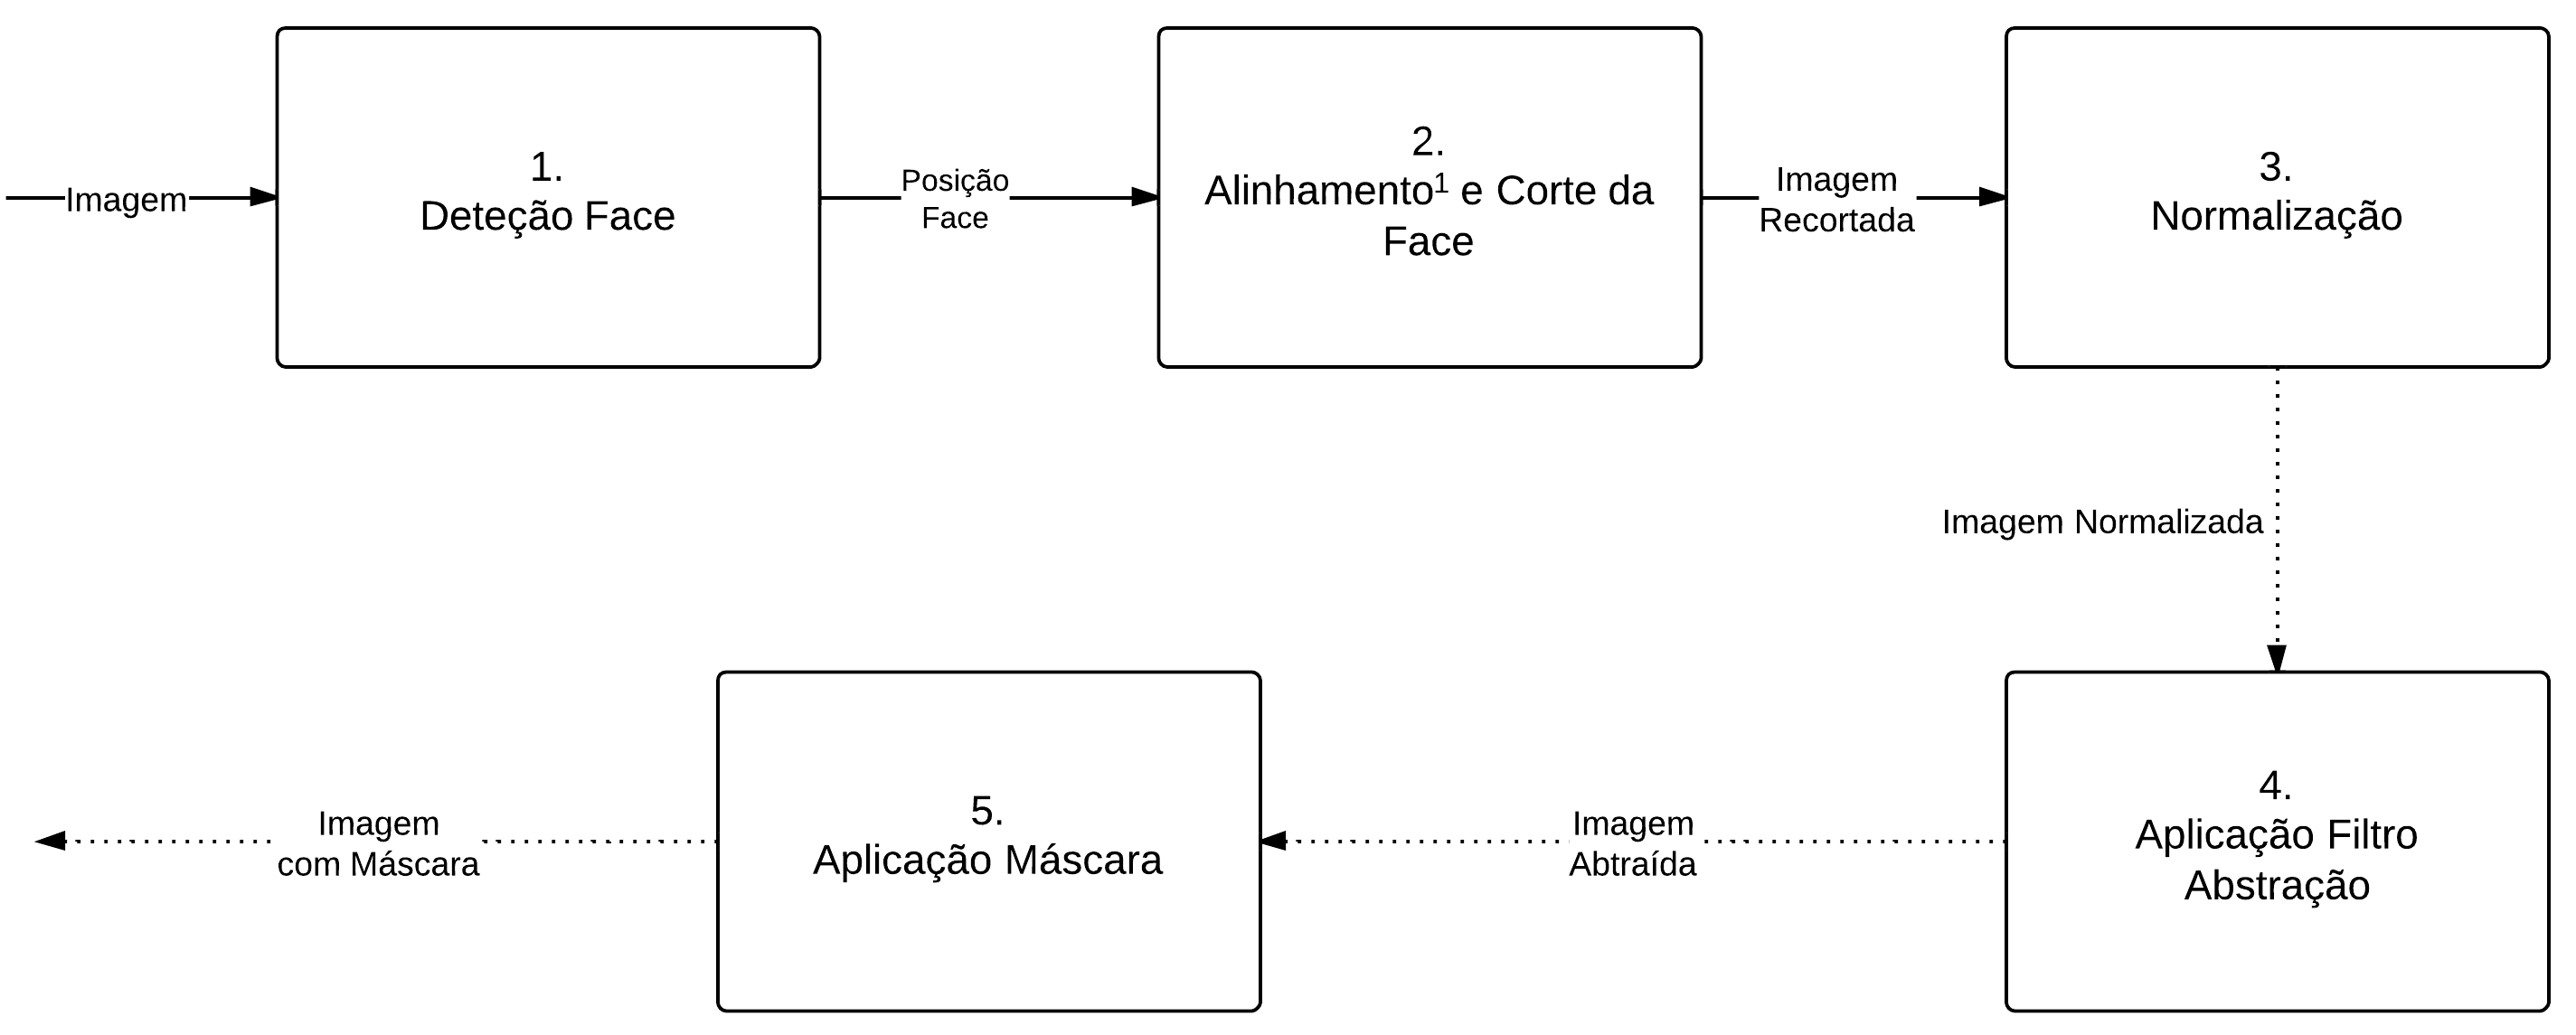
\includegraphics[width=1\textwidth]{PreProcessamentoVisage}
    \caption{Tarefas de pré-processamento disponíveis no sistema Visage.}
    \label{fig:preprocessamento}
  \end{center}
\end{figure}


Na Figura \ref{fig:preprocessamento} encontram-se representadas as tarefas de pré-processamento disponíveis no sistema de reconhecimento facial Visage, assim como a ordem pela qual as mesmas são aplicadas. As etapas de normalização, aplicação do filtro de abstração e aplicação da máscara constituem tarefas de pré-processamento opcionais pelo que se encontram representadas por uma linha a tracejado. As etapas de pré-processamento opcionais são independentes entre si, existindo assim a possibilidade de não aplicar uma das etapas sem prejudicar as restantes.  \footnote{Tal como mencionado em \ref{sec:lfw}, na avaliação do sistema foi utilizada a versão alinhada da biblioteca LFW, designada de LFW-a, pelo que a tarefa de alinhamento das imagens não foi realizada na avaliação de desempenho reportada nesta dissertação.}

\subsection{Deteção da Face} \label{sec:detecao_face}
A existência de elementos de fundo numa imagem produz um impacto significativo nos resultados obtidos por sistemas de reconhecimento facial automático, tal como é possível observar pelos resultados obtidos no Capítulo \ref{chap:resultados} e em estudos efetuados anteriormente \cite{Kumar2009}, pelo que a deteção da zona de uma imagem onde se encontra representada a face a identificar é fundamental para um bom desempenho do sistema criado. A fase de pré-processamento implementada no sistema Visage tem então como objetivo, para uma dada imagem fornecida ao sistema, determinar qual a zona da imagem onde se encontra a face a identificar.

A deteção facial é efetuada com recurso um classificador em cascata, designado de \textit{boosted cascade classifier},  treinado especificamente para a deteção de faces. O classificador utilizado encontra-se implementado na biblioteca \textit{OpenCV} e baseia-se nos trabalhos de Viola e Jones \cite{Viola2001} e posteriores melhorias introduzidas por Lienhart, Kuranov e Pisarevsky \cite{Lienhart2003}.

Um classificador é treinado com algumas centenas de imagens, de um objeto particular, neste caso uma face em posição frontal, designando-se essas imagens de exemplos positivos; assim como algumas imagens arbitrárias e não relacionadas, designadas de exemplos negativos. Quer os exemplos negativos, quer os positivos são previamente escalados para o mesmo tamanho. Após o treino, o classificador é capaz de determinar numa região de igual tamanho às imagens utilizadas no seu treino, designada de janela, se existe de uma face. Para efetuar a pesquisa de faces em toda a imagem a janela do classificador é movida ao longo da imagem de forma a que toda a área existente seja pesquisada. Para a pesquisa de faces de diferentes tamanhos é possível escalar o classificador, efetuando o varrimento da imagem nas diversas escalas que se pretende pesquisar.

Um dos principais contributos de Viola e Jones para a construção de um sistema de deteção facial eficaz é a utilização de um algoritmo de aprendizagem, designado de \textit{Adaboost}, que efetua a seleção de um número de características visuais críticas comuns a um conjunto alargado de imagens, permitindo assim a extração de pormenores essenciais para a classificação de um tipo de objeto \cite{Viola2001}. Desta forma é possível a criação de vários classificadores simples focados em características específicas da imagem. A palavra "\textit{boosted}" no classificador utilizado deriva da utilização desta técnica no mesmo.
 
A designação de classificador em cascata deriva da utilização de um conjunto de classificadores simples, de forma sequencial e combinada. Para a determinação da existência de uma face, todos os classificadores utilizados  têm de aprovar a existência da mesma, caso contrário a face é rejeitada. Um exemplo básico de um classificador seria uma árvore de decisão com pelo menos duas folhas.

No sistema Visage é utilizado um classificador facial, disponibilizado pela biblioteca \textit{OpenCV}, treinado através das características obtidas pela extração das \textit{Local Binary Patterns} \cite{Ahonen2006} de um conjunto de imagens de caras frontais. Contudo, a implementação existente na biblioteca OpenCV deste tipo de classificadores pode ser igualmente utilizada para reconhecer qualquer tipo de objetos para os quais exista informação de treino disponível.

\subsubsection*{Remoção de Conflitos e Falsos Positivos}

\begin{figure}[t]
        \centering
        \begin{subfigure}[b]{0.2\textwidth}
                \centering
                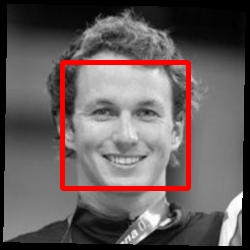
\includegraphics[width=\textwidth]{conflitos/correcta}
                \caption{Correcta}
                \label{fig:conflitos-correcta}
        \end{subfigure}%
        ~ 
        \begin{subfigure}[b]{0.2\textwidth}
                \centering
                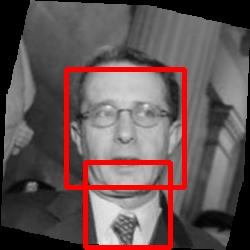
\includegraphics[width=\textwidth]{conflitos/falsos_positivos}
                \caption{Falso Positivo}
                \label{fig:conflitos-falsos_positivos}
        \end{subfigure}
        ~ 
        \begin{subfigure}[b]{0.2\textwidth}
                \centering
                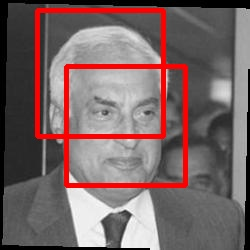
\includegraphics[width=\textwidth]{conflitos/multiplas_areas}
                \caption{Múltiplas Áreas}
                \label{fig:conflitos-multiplas_areas}
        \end{subfigure}
        ~ 
        \begin{subfigure}[b]{0.2\textwidth}
                \centering
                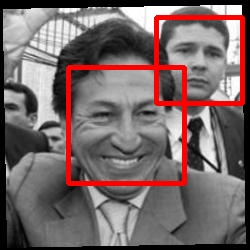
\includegraphics[width=\textwidth]{conflitos/multiplas_faces}
                \caption{Múltiplas Faces}
                \label{fig:conflitos-multiplas_faces}
        \end{subfigure}
        \caption{Comparação entre face correctamente detectada e situações de erro na detação}\label{fig:conflitos-detecao}
\end{figure}

Para uma dada imagem, a tarefa de deteção da face é responsável pela determinação de uma área de interesse, de forma rectangular, onde se encontra a face que se pretende fornecer às etapas de treino ou teste do sistema Visage. Um exemplo de uma imagem cuja face foi corretamente detetada e da respetiva área de interesse, assinada a vermelho, pode ser encontrado na Figura \ref{fig:conflitos-correcta}.

Apesar do bom desempenho do classificador utilizado na deteção das faces presentes nas imagens, existem algumas situações onde se verificou a existência de erros ou conflitos nos resultados obtidos, tal como ilustrado na Figura  \ref{fig:conflitos-detecao}. De seguida encontram-se descritas as três situações de erro encontradas:
\begin{description}
\item[Falsos Positivos] Zonas da imagem que não contém faces podem ser assinaladas como área de interesse, tal como ilustrado na Figura \ref{fig:conflitos-falsos_positivos};
\item[Múltiplas Áreas de Interesse] Para a mesma face, na análise de uma imagem são devolvidas várias regiões de interesse, tal como pode ser visto na Figura \ref{fig:conflitos-multiplas_areas};
\item[Múltiplas Faces] Na galeria utilizada para o desenvolvimento e avaliação do sistema, LFW-a, existem situaçoes onde mais do que uma pessoa se encontra representada na mesma imagem, no entanto, em cada imagem é apresentada apenas a anotação textual para a face mais relevante na fotografia, tal como pode ser visto na Figura \ref{fig:conflitos-multiplas_faces}, onde apenas a face maior possui uma anotação textual associada, pelo que apenas essa face deve ser extraída da imagem.
\end{description}

\begin{center}
\begin{table}
\begin{center}
\caption{Resultados etapa de de deteção facial para todas as pessoas com pelo menos 2 imagens na biblioteca LFW-a.}
    \begin{tabular}{ll}
    \hline
    \hline
    Pessoas                                                 & 1680                   \\
    Imagens                                                 & 9165                   \\ \hline
    Imagens com faces detectadas s/ conflito                & 95.50\% (8753 imagens) \\
    Conflitos e falsos positivos resolvidos automaticamente & 1.63\% (149 imagens)   \\
    Conflitos e falsos positivos não resolvidos (empates)   & 0.34\% (31 imagens)    \\
    Imagens com faces não detectadas                        & 2.52\% (231 imagens)   \\
    \hline
    \hline
    \end{tabular}
    \label{tab:desempenho_detecao}
\end{center}
\end{table}
\end{center}

Para a remoção dos casos de conflito observados na deteção das faces presentes na biblioteca LFW-a e ilustrados na Figura \ref{fig:conflitos-detecao}, foi adoptada a seguinte estratégia:

Para uma dada imagem é verificada a existência de uma cara usando o classificador em cascata treinado para o reconhecimento de caras frontais. Caso se verifique a deteção de um conflito, nessa imagem é necessário proceder à re-avaliação de cada uma das regiões assinaladas como área de interesse, de forma a determinar em qual se encontra a face que se pretender utilizar.

Na avaliação das várias regiões de interesse é procurada a existência de olhos, boca e nariz, com recurso a três classificadores em cascata treinados para o reconhecimento de cada um destes componentes em específico. Posteriormente é calculada uma pontuação para cada uma das regiões de interesse conforme os elementos encontrados:
\begin{itemize}
\item +100 Pontos caso sejam encontrados o par de olhos (olho esquerdo e direito) na face;
\item +50 Pontos caso seja encontrada a boca. No caso de terem sido encontrados previamente os olhos, é também verficado se distância entre a boca e os olhos é de de pelo menos 20 píxeis, de modo a garantir que um olho não é classificado como boca e vice-versa;
\item + 50 Pontos caso seja encontrado o nariz na face.
\end{itemize}
A pontuação de uma região de interesse varia assim entre os 0 e os 200 pontos. No final, é guardada apenas a região de interesse com maior pontuação. Em caso de empate, são guardadas ambas as regiões de interesse, e o utilizador do sistema é avisado do conflito, o qual deverá ser resolvido posteriormente de forma manual.

O desempenho da tarefa de deteção facial numa amostra da biblioteca LFW-a, pode ser visualizado na Tabela \ref{tab:desempenho_detecao}. Nesta amostra foram incluídas apenas as fotografias de pessoas que tenham pelos menos 2 imagens na biblioteca LFW-a, uma vez que apenas essas poderão ser utilizadas na avaliação do desempenho do sistema, utilizando, pelo menos, uma imagem para treino e uma imagem para teste. Tal como é possível observar o desempenho desta etapa é muito satisfatório, sendo que 95.5\% das faces imagens presentes nas imagens são detetadas automaticamente, às quais acrescentem 149 imagens para as quais foi possível resolver automaticamente os conflitos detetados, resultando num total de 97.13\% de faces corretamente detetadas.

\subsection{Alinhamento e Corte} \label{sec:alinhamentoEcorte}
A tarefa de deteção da face é responsável pela determinação de uma região de interesse na imagem original onde se encontra a face, sendo essa região correspondente a um retângulo tal como ilustrado na Figura \ref{fig:conflitos-correcta}. Após a deteção da região de interesse onde se encontra a face, é então possível proceder ao seu alinhamento e corte através da seguinte estratégia:

\begin{enumerate}
\item Utilizando um classificador em cascata existente na biblioteca \textit{OpenCV} é verificada a posição do olho esquerdo na região de interesse determinada para a face;
\item Utilizando um classificador em cascata existente na biblioteca \textit{OpenCV} é verificada a posição do olho direito na região de interesse determinada para a face;
\item São removidos conflitos e falsos positivos nas posições obtidas para o olho esquerdo e direito (ver Sub-secção seguinte), obtendo-se assim as duas regiões mais prováveis para cada um dos olhos;
\item É calculado o ponto central das regiões determinadas como mais prováveis para o olho esquerdo e direito, em que $p_{esquerdo}(x_1,y_1)$ corresponde ao ponto central da região detetada para o olho esquerdo, e  $p_{direito}(x_2,y_2)$ corresponde ao ponto central da região detetada para o olho direito.
\item É calculado o ângulo de rotação da imagem ($\theta$), a partir da posição determinada para os olhos:
\begin{equation}
\theta = \arctan(x_1 - x_2, y_1 - y_2)
\end{equation}
\item A imagem é rodada de acordo com o ângulo de rotação $\theta$ calculado.
\item A imagem é cortada de acordo com a região de interesse determinada na tarefa de deteção face.
\end{enumerate}

Caso não se pretenda efetuar o alinhamento da face, mas apenas a sua segmentação da restante imagem, como se verifica na utilização da galeria já alinhada, LFW-a, na avaliação do desempenho do sistema, os passos 1 a 6 são ignorados, sendo apenas segmentada a imagem de acordo com a região de interesse determinada na tarefa de deteção face. Na Figura \ref{fig:alinhamentos} encontra-se representada uma comparação entre uma imagem apenas recortada, a mesma imagem alinhada e recortada pelas estratégias acima descritas e ainda as versões LFW e LFW-a dessa imagem.

\begin{figure}[t]
        \centering
        \begin{subfigure}[b]{0.2\textwidth}
                \centering
                \includegraphics[width=\textwidth]{alinhamentos/original}
                \caption{LFW-Original}
                \label{fig:alinha_original}
        \end{subfigure}%
        ~ 
        \begin{subfigure}[b]{0.2\textwidth}
                \centering
                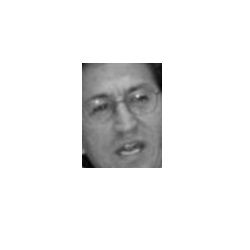
\includegraphics[width=\textwidth]{alinhamentos/nao-alinhada}
                \caption{Recortada}
                \label{fig:alinha_nao-alinhada}
        \end{subfigure}
        ~ 
        \begin{subfigure}[b]{0.2\textwidth}
                \centering
                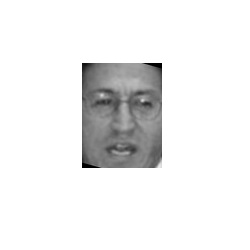
\includegraphics[width=\textwidth]{alinhamentos/alinhada}
                \caption{Alinhada}
                \label{fig:alinha_alinhada}
        \end{subfigure}
        ~ 
        \begin{subfigure}[b]{0.2\textwidth}
                \centering
                \includegraphics[width=\textwidth]{alinhamentos/lfw-a}
                \caption{LFW-a}
                \label{fig:alinha_lfw-a}
        \end{subfigure}
        \caption{Comparação entre versões original, recortada, alinhada e LFW-a.}\label{fig:alinhamentos}
\end{figure}

\subsubsection*{Remoção de Conflitos e Falsos Positivos}
Tal como explicado anteriormente, a necessidade de alinhamento de uma face previamente detetada é calculada com base na localização estimada para o seu olho esquerdo e direito e a inclinação da reta formada pela intersecção dos dois pontos centrais de cada um dos olhos. Para detetar um olho, à semelhança da estratégia adotada para detetar uma face, é utilizado um classificador em cascata que devolve uma região rectangular onde é provável a existência de um olho. 

A morfologia de um olho é um caso particularmente difícil de deteção, tendo-se registado a existência de um grande número de falsos positivos para os classificadores utilizados (olho esquerdo e direito), assim como uma má diferenciação entre o olho esquerdo, direito e a boca em algumas das imagens, pelo que a adoção de uma estratégia de remoção de conflitos se revelou essencial para a conclusão desta tarefa de pré-processamento com sucesso. A estratégia adotada foi a seguinte:

Seja $w$ a largura de uma imagem de face a alinhar e $h$ a sua altura. Sejam $c_{esquerdo}(x_1,y_1)$ e  $c_{direito}(x_2,y_2)$  os pontos correspondentes aos cantos superiores esquerdos das regiões de interesse detetadas para o olho esquerdo e direito, respetivamente, e $w_{esquerdo}$, $w_{direito}$, $h_{esquerdo}$ e $h_{direito}$ a largura e altura dessas mesmas regiões. Os conflitos entre as diversas regiões de interesse devolvidas pelos classificadores utilizados são removidos através da utilização das seguintes restrições:

\begin{itemize}
\item $x_1 < \frac{w}{4}$ e $\frac{w}{4} < x_2 < \frac{3\times w}{4}$;
\item $y_1 < \frac{h}{2}$ e $y_2 < \frac{h}{2}$;
\item $w_{esquerdo} < \frac{5\times w}{8}$ e $w_{direito} < \frac{5\times w}{8}$;
\item $h_{esquerdo} < \frac{h}{2}$ e $h_{direito} < \frac{h}{2}$;
\end{itemize}

\subsection{Normalização do Contraste} \label{sec:normalizacao}

Tal como destacado na Secção \ref{sec:sub-problemas} a tarefa de normalização encontra-se presente em alguns sistemas de reconhecimento facial automático com o objetivo de melhorar os resultados obtidos independentemente de fatores como a iluminação ou pose das faces nas imagens. A tarefa de normalização do contraste de imagem tem como objetivo normalizar a face no que diz respeito à sua iluminação e aumentar o contraste existente na mesma. De forma a tornar o sistema versátil e analisar o impacto de diferentes estratégias foram utilizadas as seguintes alternativas, ilustradas na Figura \ref{fig:normalizacao}, para a normalização do contraste:

\begin{figure}[t]
        \centering
        \begin{subfigure}[b]{0.2\textwidth}
                \centering
                \includegraphics[width=\textwidth]{normalizacao/original}
                \caption{Original               }
                \label{fig:normalizacao-original}
        \end{subfigure}%
        ~
        \begin{subfigure}[b]{0.2\textwidth}
                \centering
                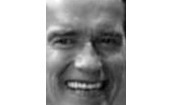
\includegraphics[width=\textwidth]{normalizacao/normalized}
                \caption{\textit{C. Streching}}
                \label{fig:normalizacao-normalized}
        \end{subfigure}
        ~ 
        \begin{subfigure}[b]{0.2\textwidth}
                \centering
                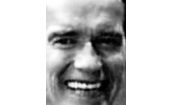
\includegraphics[width=\textwidth]{normalizacao/equalized}
                \caption{Equalização H.}
                \label{fig:normalizacao-equalized}
        \end{subfigure}
        ~
        \begin{subfigure}[b]{0.2\textwidth}
                \centering
                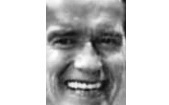
\includegraphics[width=\textwidth]{normalizacao/clahe}
                \caption{\textit{CLAHE}}
                \label{fig:normalizacao-clahe}
        \end{subfigure}
        ~ 
        \caption{Comparação entre imagem original e as várias técnicas de normalização disponíveis.}\label{fig:normalizacao}
\end{figure}

\begin{description}
\item[\textit{Contrast Streching}]
A técnica de \textit{Contrast Streching}, também designada por alguns autores simplesmente de normalização, consiste numa tentativa de alargar a gama de valores utilizados para codificar a intensidade de uma imagem de forma a que seja utilizada toda a gama de valores possíveis. No sistema desenvolvido as imagens utilizadas encontram-se convertidas para tons de cinzento, pelo que a normalização efetuada consiste num mapeamento linear dos valores originais para uma gama de intensidade entre 0 e 255. Um exemplo de uma face normalizada segundo esta estratégia pode ser visualizado na imagem \ref{fig:normalizacao-normalized}.
\end{description}

\begin{description}
\item[Equalização Histograma]
O histograma de uma imagem descreve a distribuição estatística dos níveis de intensidade de uma imagem, neste caso concreto dos níveis de cinzento, em função do seu número de píxeis. A equalização do histograma de uma imagem consiste no mapeamento das variações da escala de cinzentos de forma a que o histograma resultante se aproxime de uma outra distribuição, mais alargada e idealmente uniforme na distribuição dos valores de intensidade da imagem. Este procedimento parte do princípio de que a qualidade da imagem é uniforme em toda a imagem, aplicando um mapeamento similar a toda a imagem \cite{Bradski2008}. Um exemplo de uma imagem cujo histograma foi equalizado pode ser visto na Figura \ref{fig:normalizacao-equalized}.
\end{description}

\begin{description}
\item[\textit{CLAHE}]
\textit{Contrast limited adaptive histogram equalization (CLAHE)} procura ultrapassar as limitações da equalização de contraste, através de uma abordagem local ao problema de normalização do histograma de uma imagem. Ao contrário da abordagem tradicional apresentada acima, esta técnica tem em conta a intensidade de um conjunto de píxeis e dos seus vizinhos para a normalização do contraste e não a intensidade de toda a imagem. Para além disso, tal como o seu nome indica, esta abordagem incluí ainda um limite para o qual a equalização do histograma é realizada, evitando assim o mapeamento demasiado agressivo quando duas escalas de intensidade dispares se encontram na mesma região \cite{Reza2004}. Na Figura \ref{fig:normalizacao-clahe} encontra-se representada uma imagem resultante da sua normalização através da técnica CLAHE.
\end{description}

\subsection{Aplicação do Filtro de Abstração} \label{sec:filtros}
A quarta etapa de pré-processamento efetuada no sistema Visage corresponde à aplicação de um filtro de abstração sobre uma imagem. Os filtros de abstração constituem uma forma moderna de simplificação de conteúdo visual. A utilização destes filtros no âmbito do sistema Visage tem como objetivo analisar o seu impacto no processo de reconhecimento.

Encontram-se disponíveis três filtros, Gaussiano, Bilateral e Kuwahara Anisotrópico, os quais constituem três níveis de abstração sucessivamente mais complexos. A abstração efetuada para cada filtro encontra-se ilustrada na Figura \ref{fig:filters}, apresentado-se de seguida uma breve descrição de cada um dos filtros utilizados:

\begin{figure}[t]
        \centering
        \begin{subfigure}[b]{0.2\textwidth}
                \centering
                \includegraphics[width=\textwidth]{filters/original}
                \caption{Original}
                \label{fig:filters-original}
        \end{subfigure}%
        ~
        \begin{subfigure}[b]{0.2\textwidth}
                \centering
                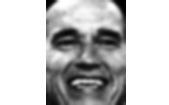
\includegraphics[width=\textwidth]{filters/gaussian}
                \caption{Gaussiano}
                \label{fig:filters-gaussian}
        \end{subfigure}
        ~ 
        \begin{subfigure}[b]{0.2\textwidth}
                \centering
                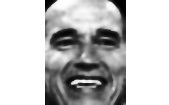
\includegraphics[width=\textwidth]{filters/bilateral}
                \caption{Bilateral}
                \label{fig:filters-bilateral}
        \end{subfigure}
        ~
        \begin{subfigure}[b]{0.2\textwidth}
                \centering
                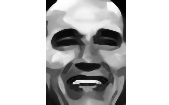
\includegraphics[width=\textwidth]{filters/akf}
                \caption{Kuwahara A.}
                \label{fig:filters-kuwahara}
        \end{subfigure}
        ~ 
        \caption{Comparação entre imagem original e os vários filtros de abstração utilizados.}\label{fig:filters}
\end{figure}

\begin{description}
\item[Filtro Gaussiano]
A aplicação de um filtro gaussiano para a suavização de uma imagem é uma técnica amplamente utilizada em áreas próximas do processamento de imagem e computação gráfica e tem como objetivo reduzir o ruído e detalhe de uma imagem. Um filtro gaussiano calcula um média pesada dos valores dos píxeis vizinhos, na qual o peso de um píxel na média diminui conforme a sua distância ao centro aumenta.

No âmbito do sistema Visage a utilização deste filtro tirou partido da implementação existente na biblioteca \textit{OpenCV}, nomeadamente a partir da função \textit{gaussianBlur}, tendo sido utilizada uma vizinhança de raio sete píxeis.

\item[Filtro Bilateral]
Tal como introduzido na Secção \ref{subsec:bilateral}, o filtro bilateral tem como objetivo suavizar as zonas com menor contraste na imagem sem afetar os limites de maior contraste, permitindo assim reduzir o ruído presente na imagem enquanto os seu contornos são preservados.

À semelhança do filtro gaussiano a utilização deste filtro foi efetuada com recurso à implementação existente na biblioteca \textit{OpenCV}, nomeadamente a partir da função \textit{bilateralFilter}, tendo sido utilizado um raio de oito píxeis vizinhos na aplicação do filtro.

\item[Filtro Kuwahara Anisotrópico]
O filtro Kuwahara Anisotrópico (FKA) é uma generalização do filtro Kuwahara (ver \ref{subsec:kuwahara}) que remove alguns artefactos originados na aplicação do filtro original através da adaptação da forma, escala e orientação do filtro à estrutura local das características da imagem \cite{Kyprianidis2009}. Desta forma é produzido um efeito de abstração tipo pintura, onde é removida informação não essencial em zonas de elevado contraste, enquanto são preservados os limites representados nas zonas de menor contraste. Por outro lado, este filtro tira partido da placa gráfica para a realização da abstração das imagens, tornando-se assim particularmente indicado para o processamento de um elevado número de fotografias.

Para a utilização deste filtro foi utilizada a implementação de Jan Kyprianidis disponível em [] \footnote{https://code.google.com/p/gpuakf/}.

\end{description}
\subsection{Aplicação de Máscara} \label{sec:mascara}

\begin{figure}[t]
        \centering
        \begin{subfigure}[b]{0.2\textwidth}
                \centering
                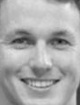
\includegraphics[width=\textwidth]{mascara/sem_mascara}
                \caption{Original}
                \label{fig:sem-mascara}
        \end{subfigure}%
        ~ ~ ~
        \begin{subfigure}[b]{0.2\textwidth}
                \centering
                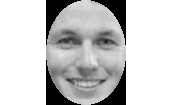
\includegraphics[width=\textwidth]{mascara/com_mascara}
                \caption{Recortada}
                \label{fig:com-mascara}
        \end{subfigure}
        ~ 
        \caption{Exemplo de face já segmentada, com e sem máscara.}\label{fig:mascara}
\end{figure}

A existência de fundo e elementos externos à face numa imagem pode afetar significativamente os resultados obtidos no seu reconhecimento ao permitir que um conjunto de imagens com fundos semelhantes possam ser identificadas como pertencendo à mesma pessoa não pela face representada na imagem, mas pelos elementos presentes no fundo da mesma. A aplicação de uma máscara elíptica sobre face visa a remoção do fundo ainda existente na imagem após a deteção e segmentação da face e eventuais tarefas de pré-processamento realizadas.

Um exemplo de uma imagem antes e depois da aplicação da máscara pode ser visto em \ref{fig:mascara}. A estratégia de aplicação de uma máscara para melhoria dos resultados obtidos no reconhecimento facial já foi aplicada com sucesso anteriormente em diversas situações, como são exemplo a avaliação FERET \cite{Phillips2000} ou o trabalho realizado por Ahonen \textit{et al.} \cite{ahonen2004face}.

\section{Módulo \textit{FaceModel}} \label{sec:facemodel}
O módulo \textit{FaceModel} constitui uma camada de nível superior implementada para encapsular a comunicação com o módulo de reconhecimento facial disponível na biblioteca \textit{OpenCV}, designado \textit{FaceRecognizer}, assim como estender algumas das funcionalidades do mesmo. 

As principais responsabilidades do módulo \textit{FaceModel} consistem em treinar um modelo de reconhecimento facial, assim como determinar para uma dada imagem qual a sua identificação mais provável, ou qual o conjunto ordenado de identificações mais prováveis a partir do modelo criado.

O modelo de reconhecimento facial pode ser criado com três algoritmos de reconhecimento facial, \textit{Eigenfaces}, \textit{Fisherfaces} e \textit{LBPH}, implementados na biblioteca \textit{OpenCV} e descritos em mais pormenor nas Secções \ref{sec:eigen}, \ref{sec:fisher} e \ref{sec:lbph}, respetivamente. Uma vez treinado um modelo é também possível armazenar o mesmo num ficheiro e efetuar o seu carregamento posteriormente, evitando assim um novo treino, o qual dependendo do número de imagens a treinar pode revelar-se computacionalmente custoso.

As funcionalidades disponíveis na biblioteca \textit{OpenCV} para os três algoritmos foram expandidas de forma a permitir que, para uma dada imagem fornecida ao sistema, seja devolvida uma lista ordenada, por ordem decrescente de similaridade, de entidades. Desta forma é possível para além de identificar a pessoa presente numa imagem, dizer qual a lista de pessoas que mais se parecem com a pessoa representada na imagem. Uma descrição detalhada da expansão efetuada às funcionalidades disponíveis na biblioteca OpenCV pode ser encontrada em \ref{sec:topn}.

\subsection{\textit{Eigenfaces}} \label{sec:eigen}
O método \textit{Eigenfaces} foi introduzido por Turk e Pentland em 1991 \cite{Turk1991}, e tira partido da Análise dos Componentes Principais (\textit{Principal Component Analysis - PCA}) para efetuar o reconhecimento facial automático.

A análise de componentes principais tem como objetivo determinar as relações existentes entre diferentes conjuntos de dados, nomeadamente ao nível das suas diferenças e semelhanças, tirando partido da redundância existente para criar uma representação reduzida dos dados sem que a perda de informação ocorrida seja significativa. As imagens faciais possuem uma grande redundância natural. O algoritmo \textit{Eigenfaces}, através da análise dos componentes principais dessas imagens, efetua uma projeção das imagens faciais num sub-espaço onde se evidenciam apenas as variações entre as diversas caras conhecidas pelo sistema.

A redução do espaço de representação é importante no problema de reconhecimento facial em imagens, devido à grande dimensionalidade exigida para a representação de uma face. Considerando, por exemplo, uma imagem de apenas $256 \times 256$ píxeis, essa imagem é traduzida por um espaço vetorial de $n \times m$ píxeis, necessitando de um total de $65536$ píxeis para ser representada.

O processo de reconhecimento facial com recurso ao algoritmo \textit{Eigenfaces} consiste nos seguintes passos:
\begin{enumerate}
\item Seleção de um conjunto de dados iniciais (conjunto de treino);
\item Projeção dos dados obtidos num sub-espaço de faces através da ACP;
\item Seleção de uma imagem a reconhecer;
\item Projeção da face a reconhecer no sub-espaço do conjunto de treino, calculando as distâncias obtidas para cada face conhecida pelo sistema;
\item Determinar qual a face do conjunto de treino com menor distância à face a reconhecer;
\item Caso a distância para a face obtida seja menor do que um limite operacional estabelecido, a imagem é reconhecida como sendo essa pessoa, caso contrário, a face é identificada como sendo uma pessoa desconhecida pelo sistema.
\end{enumerate}

Este método efetua uma abordagem holística ao problema de reconhecimento facial em imagens, uma vez que tem em consideração a representação facial como um todo, não fazendo a distinção entre pontos específicos da face como olhos, orelhas ou nariz para efetuar o reconhecimento facial. Uma vantagem deste tipo de representação é a reduzida sensibilidade ao ruído presente nas imagens \cite{Zhao2003}.

\subsection{\textit{Fisherfaces}} \label{sec:fisher}
A análise dos componentes principais visa determinar o sub-espaço onde se verifica uma maior variação entre um conjunto de imagens. No entanto, a variação na representação facial de uma pessoa encontra-se muitas vezes relacionada com mudanças de expressões faciais ou iluminação dos indivíduos. O sub-espaço criado pelo algoritmo \textit{Eigenfaces} não traduz muitas vezes apenas as diferenças de identidade entre os diversos indivíduos, mas também as diferenças verificadas entre as várias representações de um indivíduo devido à variação nas condições de captura das imagens. O algoritmo \textit{Fisherfaces} \cite{Belhumeur1997, Etemad1997, Zhao1998}, tenta resolver este problema, através da aplicação de um passo de Análise Linear Discriminante (\textit{Linear Discriminant Analysis - LDA}) após a análise dos componentes principais, de forma a determinar mais corretamente as variações intra-classe existentes no conjunto de imagens a avaliar.

A LDA, inicialmente introduzida por Fisher em 1936 \cite{FISHER1936}, tenta maximizar as diferenças existentes entre diferentes indivíduos(inter-classe) e minimizar as variações entre imagens da mesma pessoa(intra-classe) de modo a obter uma representação mais robusta em termos de variação ao nível da iluminação. Após a aplicação dos passos de PCA e LDA, o processo de reconhecimento do método \textit{Fisherfaces} é semelhante ao efetuado pelo método \textit{Eigenfaces}, sendo também efetuada uma abordagem holística ao reconhecimento facial.


\subsection{\textit{Local Binary Patterns Histograms (LBPH)}} \label{sec:lbph}
Ao contrário dos algoritmos descritos anteriormente, o LBPH efetua uma abordagem local ao problema de reconhecimento facial, efetuando uma extração das características locais de uma imagem. Este tipo de abordagem possui a vantagem de possuir uma baixa dimensionalidade implícita, pelo que não existe a necessidade de efetuar a projeção das imagens num sub-espaço.

A ideia base das \textit{Local Binary Patterns (LBP)}, consiste em resumir a estrutura local de uma imagem através de uma comparação de um píxel com os seus vizinhos. Dado um píxel central é analisada a diferença entre esse píxel e cada um dos seus vizinhos. Se a intensidade do píxel for maior ou igual do que a do seu vizinho é atribuído o valor 1, caso contrário é atribuído o valor 0. Cada píxel pode então ser traduzido por um número binário do género $11001111$. Dados $8$ píxeis é então possível efetuar $2^8$ combinações, cada uma designada de LBP.

Ahonen \textit{et al.} \cite{ahonen2004face}, propuseram o uso de LBP para o reconhecimento facial em imagens. A sua abordagem consiste na divisão da face em pequenas regiões das quais são derivadas LBP e concatenadas numa representação única designada de LBPH, a qual representa uma imagem facial. O reconhecimento é depois efetuado através do determinação do vizinho mais próximo no espaço de faces computado.

\subsection{Top $N$ Resultados} \label{sec:topn}
Após o treino do sistema, a identificação de uma imagem é obtida de forma semelhante para os três algoritmos disponíveis, e pode ser resumida no seguinte conjunto de passos:
\begin{enumerate}
\item É criada uma representação de baixo nível da imagem a identificar, aqui designada de prova.
\item A prova é comparada com cada uma das representações de baixo nível criadas durante o treino do sistema e às quais se encontra associado um código numérico representativo da pessoa associada a essa representação.
\item É devolvida o código da pessoa correspondente à menor distância entre a prova e a representação de baixo nível treinada.
\end{enumerate}

Para os algoritmos \textit{Eigenfaces} e \textit{Fisherfaces} a representação de baixo nível de uma imagem corresponde à projeção desta no sub-espaço de imagens criado com a análise dos componentes principais, no caso do \textit{Eigenfaces}, e com a posterior análise linear discriminante, no caso do \textit{Fisherfaces}. A comparação entre a prova e as representações de baixo nível criadas no treino é efetuada em ambos os casos através da distância euclidiana entre as matrizes das duas representações.

Para o algoritmo \textit{LBPH} a representação de baixo nível criada corresponde ao histograma representativo das \textit{local binary patterns} de uma imagem. A comparação entre a prova e as representações de baixo nível criadas durante o treino é efetuada através da comparação da distância entre os seus histogramas.

A extensão efetuada à implementação existente na biblioteca \textit{OpenCV} incide sobre o ponto 3 dos passos acima citados. Em vez de apenas ser devolvido o código identificativo da pessoa cuja representação apresenta uma menor distância às representações de baixo nível existentes, é devolvida uma lista de $n$ elementos, ordenada de forma crescente pelas distâncias calculadas. Esta lista encontra-se agrupada pelas diferentes entidades, significando assim que cada pessoa apenas aparece uma única vez na lista, independentemente da existência de várias representações de baixo nível referentes a essa pessoa. Com a extensão implementada torna-se possível o desenvolvimento de aplicações que para uma imagem fornecida respondam à pergunta "Qual é nome das 10 pessoas mais parecidas com a imagem fornecida?", em vez de apenas "Qual é a pessoa mais parecida com a imagem fornecida?".

\section{Funcionalidades} \label{sec:funcionalidades}
O desenvolvimento do sistema Visage resultou na criação de cinco aplicações com diferentes funcionalidades e responsabilidades no âmbito deste sistema. Todas as aplicações que seguem um paradigma de caixa preta, no qual para um conjunto de dados de entrada é produzido um resultado específico. 

As primeiras três aplicações desenvolvidas, \textit{FaceDetector.exe}, \textit{FaceRecognizer.exe} e \textit{CSVCreator.exe} foram criadas com o objetivo de efetuar a avaliação de desempenho do sistema reportada no Capítulo \ref{chap:resultados}. Nesta avaliação é efetuada uma análise do impacto da abstração de imagens e outras tarefas de pré-processamento no processo de reconhecimento facial automático.

As aplicações \textit{TrainAndSaveModel.exe} e \textit{TopN.exe} permitem a utilização do sistema Visage como base de outros programas que tirem partido do reconhecimento facial de imagens no seu funcionamento.

\begin{description}
\item[FaceDetector.exe] Efetua o pré-processamento de uma galeria de imagens de acordo com os seguintes argumentos:

\begin{itemize}
\item \textbf{\textit{libraryPath.txt}}: O ficheiro txt com a descrição das imagens da galeria a processar.
\item \textbf{\textit{outputDirName}}: O caminho do novo diretório a criar.
\item \textbf{-mask}: Define se deve ser colocada uma máscara sobre a imagem (ver \ref{sec:mascara}). Parâmetro opcional.
\item \textbf{\textit{-N, -E ou -C}}: Define qual o tipo de normalização que deve ser efetuada sobre a imagem, \textit{-N}, \textit{-E} ou \textit{-C} para as técnicas \textit{Contrast Streching}, Equalização Histograma e CLAHE, respetivamente (ver \ref{sec:normalizacao}). Parâmetro opcional.
\item \textbf{\textit{-G ou -B}}: Define qual o filtro de abstração a aplicar sobre a imagem, -G ou -B, para os filtros gaussiano ou bilateral, respetivamente. Para efetuar o pré-processamento com recurso ao filtro kuwahara anisotrópico é necessário recorrer a um programa externo (ver \ref{sec:filtros}). Parâmetro opcional.
\item \textbf{\textit{-align}}: Define se deve ser efetuado alinhamento das faces detetadas nas imagens (ver \ref{sec:alinhamentoEcorte}). Parâmetro opcional.
\end{itemize}

\item[FaceRecognizer.exe] Efetua a avaliação do desempenho do sistema de reconhecimento facial para uma determinada galeria, de acordo com os seguintes parâmentros:

\begin{itemize}
\item \textbf{\textit{libraryPath.txt}}: O ficheiro txt com a descrição das imagens da galeria a processar.
\item \textbf{\textit{results.txt}}: O ficheito txt com os resultados da avaliação efetuada num formato legível para humanos.
\item \textbf{\textit{-E, -F ou -L}}: Define qual o algoritmo de reconhecimento facial a utilizar -E, -F ou -L para \textit{Eigenfaces}, \textit{Fisherfaces} ou \textit{LBPH} (ver \ref{sec:facemodel}).
\item \textbf{\textit{nResults }}: Define o número de rankings máximo a avaliar.
\end{itemize}

\item[CSVCreator.exe] Permite criar novas sub-galerias a partir de outras pré-existentes, assim como computar as estatísticas de uma galeria, de acordo com os seguinte parâmetros:

\begin{itemize}
\item \textbf{\textit{libraryPath.txt}}: O ficheiro txt com a descrição das imagens da galeria original.
\item \textbf{\textit{outputfilename}}: O nome do ficheiro com a descrição da sub-galeria criada.
\item \textbf{\textit{bottomLimit}}: O número de mínimo de imagens por pessoa.
\item \textbf{\textit{topLimit}}: O número de máximo de imagens por pessoa.
\item \textbf{\textit{statsFile}}: Nome do ficheiro onde ficam armazenadas as estatísticas de uma galeria.
\end{itemize}

\item[TrainAndSaveModel.exe] Permite treinar um modelo de reconhecimento facial de uma galeria passada como argumento e gravar esse modelo para um ficheiro para posterior utilização.

\begin{itemize}
\item \textbf{\textit{libraryPath.txt}}: O ficheiro txt com a descrição das imagens da galeria a processar.
\item \textbf{\textit{percentageToTrain}}: A percentagem de imagens de cada pessoa a usar como imagem de treino e teste.
\item \textbf{\textit{-E, -F ou -L}}: Define qual o algoritmo de reconhecimento facial a utilizar -E, -F ou -L para \textit{Eigenfaces}, \textit{Fisherfaces} ou \textit{LBPH} (ver \ref{sec:facemodel}).
\item \textbf{\textit{output.xml}}: O ficheiro onde deve ser gravado o modelo treinado.
\end{itemize}

\item[TopN.exe] Devolve o nomes das \textit{n} personalidades mais parecidas com a personalidade representada na imagem. Efetua o pré-processamento da imagem passada como argumentos, com aplicação de máscara, normalização através de equalização do histograma e alinhamento da face.

\begin{itemize}
\item \textbf{\textit{imagePath}}: O caminho da imagem a reconhecer.
\item \textbf{\textit{model.xml}}: O modelo de reconhecimento facial previamente treinado a utilizar.
\item \textbf{\textit{nResults}}: O número de elementos máximo a incluir no top de resultados devolvido.
\end{itemize}

\end{description}